Для построения классификатора Random Forest (см. раздел~\ref{random_forest}) необходимы два параметра, которые изначально неизвестны: количество деревьев решений ($ n $), на основе которых будет производиться классификация, а также число признаков ($ m $), выбираемых случайным образом из начального набора признаков для построения деревьев решений.

Оптимальные значения данных параметров могут быть подобраны в ходе вычислительных экспериментов с помощью ошибки Out-Of-Bag --- встроенной несмещенной оценки алгоритма Random Forest Classifier, вычисляемой на основе примеров, не вошедших в случайную подвыборку на этапе построения дерева решений. Ошибка Out-Of-Bag усредняется для всех деревьев решений в Random Forest.~\cite{random_forest}

Для подбора оптимальных значений параметров классификатора были проведены вычислительные эксперименты, в ходе которых вычислялась минимальная ошибка Out-Of-Bag при различных значениях деревьев (от 10 до 100) и при трех раличных значениях количества признаков (рис.~\ref{3:3}). Результаты вычислений приведены в таблице~\ref{tab:6}, на основании которых можно сделать вывод, что оптимальным значением количества случайно выбираемых признаков является квадратный корень из N, где N --- это общее количество признаков. При этом, как видно на рисунка~\ref{3:3}, ошибка классификации для $ m = \sqrt{N} $ cнижается при приближении числа деревьев решений к 100. Таким образом для дальнейших вычислений в качестве оптимальных параметров классификатора были взяты значения $ m = \sqrt{N} $ и $ n = 100 $.


\begin{figure}[h!]
\center{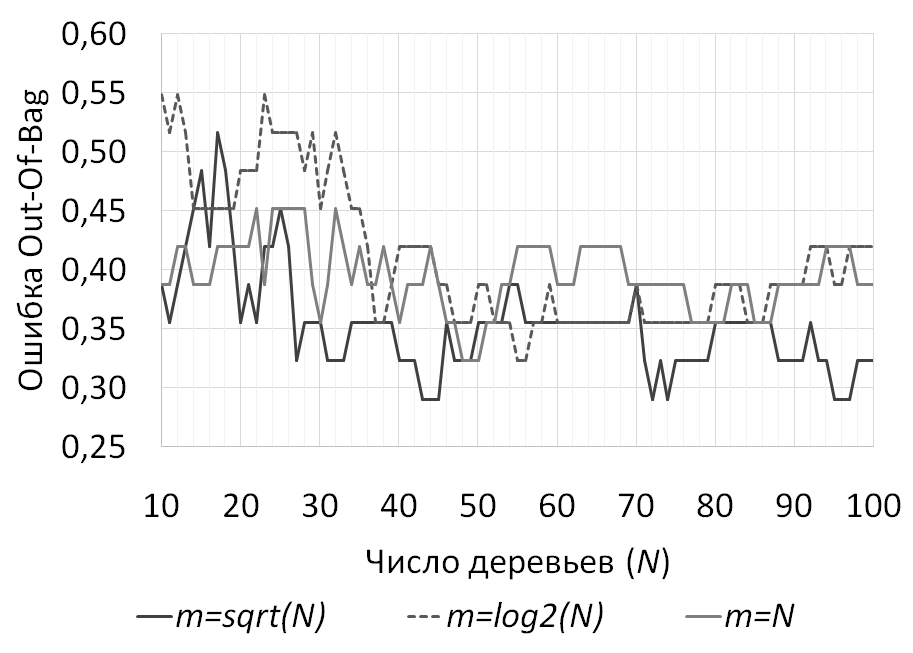
\includegraphics[width=0.6\linewidth]{3}}
\caption{ Результат вычисления ошибки Out-Of-Bag }
\label{3:3}
\end{figure} 

\begin{table}[h!]
\caption{ Вычисление оптимального количества деревьев ($ m $) и признаков ($ n $) }
\label{tab:6}
\begin{center}
\begin{tabularx}{\linewidth}{|X|X|X|X|X|X|X|}
\hline
 & \multicolumn{2}{|c|}{$ m = \sqrt{N} $} & \multicolumn{2}{|c|}{$ m = log_{2}(N) $} & \multicolumn{2}{|c|}{$ m = N $} \\
\hline
MIN & n & oob\_error & n & oob\_error & n & oob\_error \\
\hline
1 & 40 & 0,290 & 53 & 0,226 & 36 & 0,290\\
\hline
2 & 18 & 0,323 & 100 & 0,323 & 38 & 0,194 \\
\hline
3 & 60 & 0,226 & 34 & 0,355 & 10 & 0,355 \\
\hline
4 & 77 & 0,258 & 42 & 0,355 & 12 & 0,290 \\
\hline
5 & 78 & 0,194 & 91 & 0,290 & 16 & 0,323 \\
\hline
Ср. & 55 & 0,258 & 64 & 0,310 & 23 & 0,290 \\
\hline
\end{tabularx}
\end{center}
\end{table}
